\documentclass[a4paper,12pt]{book}

\usepackage{packages}
% Documentation:
% http://anorien.csc.warwick.ac.uk/mirrors/CTAN/macros/latex/contrib/titlesec/titlesec.pdfhttp://anorien.csc.warwick.ac.uk/mirrors/CTAN/macros/latex/contrib/titlesec/titlesec.pdf

% chapter title
\titleformat{\chapter} % command
[display] % shape
{\normalfont\huge\bfseries\color{Prune}\centering} % format
{} % label
{0pt} % sep
{\Huge} % before-code
{} % after-code

\titlespacing*{\chapter} % command
{0pt} % left
{50pt} % before-sep
{40pt} % after-sep
{} % right-sep

% Documentation:
% https://texlive.mycozy.space/macros/latex/contrib/mdframed/mdframed.pdf
\usepackage{mdframed}
% chapter abstract environment
\newmdenv[
	backgroundcolor=lightgrey,
	linecolor=Prune,
	innerleftmargin=10pt,
	innerrightmargin=10pt,
	innertopmargin=10pt,
	innerbottommargin=10pt,
	%nobreak=true,
	skipabove=1cm,
	frametitle={\color{Prune}Abstract}, % Title text
	frametitlefont={\bfseries}, % Font settings for the title
	frametitlealignment=\centering, % Centers the title
	]
{chapterabstract}

% Documentation:
% https://mirrors.mit.edu/CTAN/macros/latex/contrib/etoc/etoc.pdf
\usepackage{etoc} % for local ToC
% show global content up to:
% -2: book
% -1: part
%  0: chapter
%  1: section
%  2: sub-section
%  3: sub-sub-sections
%  4: paragraph
%  5: sub-paragraph
\etocsettocdepth{1}
\setcounter{secnumdepth}{3}

% chapter style table of content
\def \chapterStyleToC{
	% add separation bar above and below local ToC
	\etocsettocstyle{
		\noindent\rule{\textwidth}{0.5pt}
		\vspace{5mm}
	}{
		\vspace{5mm}
		\noindent\rule{\textwidth}{0.5pt}
	}
	% show local content up to:
	\etocsettocdepth{2}
}

% centered figures captions
\captionsetup{justification=centering,margin=2cm}
\graphicspath{
	{./1_background/}
	{./2_introduction/}
	{./3_dosimetry_optimization/}
	{./4_doses_relations/}
	{./5_automation_classic/}
	{./6_automation_mimicking/}
	{./7_conclusion/}
	{./../}
}


\begin{document}
	% titles
\def \englishtitle {Methods for automatization of the dosimetry for radiotherapy treatments.}
\def \frenchtitle {Méthodes pour l'automatisation de la dosimetrie pour les traitements radiothérapiques.}

% PhD details
\def \specialty {Spécialité de doctorat: ...}
\def \doctoralSchool {École doctorale n$^{\circ}$ 573 Interfaces : matériaux, systèmes, usages, ED INTERFACE}
\def \graduateSchool {Graduate School: Sciences de l’Ingénierie et des Systèmes, SIS}

\def \researchUnits {
	\textbf{Radiothérapie} (Institut Régionale du Cancer de Montpellier), \textbf{Advanced Research} (TheraPanacea), et \textbf{MICS, Mathématiques et Informatique pour la Complexité et les Systèmes} (Université Paris-Saclay, CentraleSupélec)
}
\def \directors {
	\textbf{Nikos Paragios}, Professeur, et la co-direction de \textbf{Paul-Henry Cournède}, Professeur
}

\def \date {JJ mois AAAA}
\def \author{Paul Raymond François DUBOIS}

\def \jury {
	\textbf{Prénom NOM} & Président ou Présidente\\
	Titre, Affiliation & \\
	\textbf{Prénom NOM} & Rapporteur \& Examinateur / trice \\
	Titre, Affiliation & \\
	\textbf{Prénom NOM} & Rapporteur \& Examinateur / trice \\
	Titre, Affiliation & \\
	\textbf{Prénom NOM} & Examinateur ou Examinatrice \\
	Titre, Affiliation & \\
	\textbf{Prénom NOM} &  Examinateur ou Examinatrice \\
	Titre, Affiliation & \\
}
	\begin{titlepage}
	
	%\thispagestyle{empty}
	
	\newgeometry{left=6cm,bottom=2cm, top=1cm, right=1cm}
	
	\tikz[remember picture,overlay] \node[opacity=1,inner sep=0pt] at (-13mm,-135mm){
\includegraphics{preamble/Frame-ups.pdf}};
	
	%*****************************************************
	%******** NUMÉRO D'ORDRE DE LA THÈSE À COMPLÉTER *****
	%******** POUR LE SECOND DÉPOT                   *****
	%*****************************************************
	
	\color{white}
	
	\begin{picture}(0,0)
		\put(-152,-743){\rotatebox{90}{\Large \textsc{THESE DE DOCTORAT}}} \\
		\put(-120,-743){\rotatebox{90}{NNT : 2020UPASA001}}
	\end{picture}
	
	%*****************************************************
	%**  LOGO  ÉTABLISSEMENT PARTENAIRE SI COTUTELLE
	%**  CHANGER L'IMAGE PAR DÉFAUT **
	%*****************************************************
	\vspace{-1mm} % à ajuster en fonction de la hauteur du logo
	%\flushright \includegraphics[scale=1]{logo2.png}
	
	%*****************************************************
	%******************** TITRE **************************
	%*****************************************************
	
	\flushright
	\vspace{10mm} % à régler éventuellement
	\color{Prune}
	
	\fontsize{22}{26}\selectfont
	\Huge \frenchtitle \\
	
	\normalsize
	\color{black}
	\Large{\textit{ \englishtitle }} \\
	%*****************************************************
	
	
	\fontsize{8}{12}\selectfont
	
	\vspace{1.5cm}
	
	\normalsize
	\textbf{Thèse de doctorat de l'université Paris-Saclay} \\
	
	\vspace{6mm}
	
	\small \specialty \\
	\small \doctoralSchool \\
	\small \graduateSchool \\
	\vspace{6mm}
	
	\footnotesize Thèse préparée dans les unités de recherche \researchUnits, sous la direction de \directors\\
	\vspace{15mm}
	
	\textbf{Thèse soutenue à Paris-Saclay, le JJ mois AAAA, par}\\
	\bigskip
	\Large {\color{Prune} \textbf{ \author }} % Changer le Prénom et le NOM
	
	%************************************
	\vspace{\fill} % ALIGNER LE TABLEAU EN BAS DE PAGE
	%************************************
	
	\bigskip
	
	\flushleft
	\small {\color{Prune} \textbf{Composition du jury}}\\
	{\color{Prune} \scriptsize {Membres du jury avec voix délibérative}} \\
	\vspace{2mm}
	\scriptsize
	\begin{tabular}{|p{7cm}l}
		\arrayrulecolor{Prune}
		\textbf{Prénom NOM} &   Président ou Présidente\\ 
		Titre, Affiliation & \\
		\textbf{Prénom NOM} &  Rapporteur \& Examinateur / trice \\ 
		Titre, Affiliation   &   \\ 
		\textbf{Prénom NOM} &  Rapporteur \& Examinateur / trice \\ 
		Titre, Affiliation  &   \\ 
		\textbf{Prénom NOM} &  Examinateur ou Examinatrice \\ 
		Titre, Affiliation   &   \\ 
		\textbf{Prénom NOM} &  Examinateur ou Examinatrice \\ 
		Titre, Affiliation   &   \\ 
		
		
	\end{tabular} 
	
\end{titlepage}
	% page of summaries to keep on the 2nd page
% if the summaries are too long to fit on a single page, put one summary per page
\thispagestyle{empty}
\newgeometry{top=1.5cm, bottom=1.25cm, left=2cm, right=2cm}

\noindent 

\includegraphics[height=2.45cm]{preamble/ed-interfaces.png}
\vspace{1cm}

\small

\begin{mdframed}[linecolor=Prune,linewidth=1]
	
	\textbf{Titre:} \frenchTitle
	
	\vspace{1mm} \noindent
	\textbf{Mots clés:} \frenchKeyWords 
	
	\begin{multicols}{2}
		\textbf{Résumé:} \\
		\frenchAbstract
	\end{multicols}
	
\end{mdframed}

\vspace{1cm}
\Needspace{12cm}

\begin{mdframed}[linecolor=Prune,linewidth=1]
	
	\textbf{Title:} \englishTitle
	
	\vspace{1mm} \noindent
	\textbf{Keywords:} \englishKeyWords
	
	\begin{multicols}{2}
		\textbf{Abstract:} \\
		\englishAbstract
	\end{multicols}
\end{mdframed}



\newgeometry{top=4cm, bottom=4cm, left=2cm, right=2cm}
	
	\pagenumbering{roman}	
	\chapter*{Acknowledgments}
%I have sometimes felt alone during those three year, but I came to realize that if I couldn't name people supporting me, it was not because they were too few, but too many.
%This section is dedicated to all those who indirectly contributed to this manuscript.
%
%I have sometimes felt alone during those three years, but I realized that if I couldn't name people supporting me, it was not because they were too few but too many.
%This section is dedicated to all those who indirectly contributed to this manuscript.

%During those three years, I often felt alone.
%But I eventually realized that the challenge wasn't in finding people who supported me, but in naming them all; there were simply too many.
%This section is dedicated to everyone who, in their own way, contributed to this manuscript.

%During those three years, I often felt alone.
%But I eventually realized that the challenge wasn't finding people who supported me, but naming them all; there were too many.
%This section is dedicated to everyone who, in their way, contributed to this manuscript.

%During those three years, I often felt alone, but I eventually realized that the reason I couldn't name everyone who supported me wasn't because there were too few, but because there were so many.
%This section is dedicated to all those who, in their own way, contributed to this manuscript.

During those three years, I often felt alone, but I eventually realized that I couldn't name everyone who supported me not because there were too few, but because there were so many.
This section is dedicated to all those who contributed to this manuscript.

[...]
	\chapter*{List of contributions}
\subsection*{Publication}
\subsubsection*{Full-length Article}
\begin{itemize}
	\item "Radiotherapy dose optimization via clinical knowledge based reinforcement learning",
	Paul Dubois, Paul-Henry Cournède, Nikos Paragios, and Pascal Fenoglietto,
	\textit{Artifcial Intelligence in Medicine} (AIME), 2024
\end{itemize}

\subsubsection*{Full-length Presentation}
\begin{itemize}
	\item "Dose Volume Histograms Guided Deep Dose Predictions",
	Paul-Henry Cournède Nikos Paragios Paul Dubois, Carlos Santos Garcia and Pascal Fenoglietto,
	\textit{Société Française de Physique Médicale} (SFPM), 2024, Dijon, France
	
	\item "Radiotherapy dose optimization via clinical knowledge based reinforcement learning",
	Paul Dubois, Paul-Henry Cournède, Nikos Paragios, and Pascal Fenoglietto,
	\textit{Artifcial Intelligence in Medicine} (AIME), 2024, Salt Lake City, Utha, USA
\end{itemize}

\subsubsection*{Poster Presentation}
\begin{itemize}
	\item "A Novel Framework for Multi-Objective Optimization and Robust Plan Selection Using Graph Theory",
	Paul Dubois, Carlos Santos Garcia, Paul-Henry Cournède, Nikos Paragios, and Pascal Fenoglietto,
	\textit{Société Française de Physique Médicale} (SFPM), 2024, Dijon, France
	
	\item "Clinically Dependent Fully Automatic Treatment Planning System",
	Paul Dubois, Pascal Fenoglietto, Paul-Henry Cournède, and Nikos Paragyos.
	\textit{American Society for Radiation Oncology} (ASTRO), 2024, Dijon, France
	
	\item "Attention mechanism on dose-volume histograms for deep dose predictions",
	Paul-Henry Cournède Pascal Fenoglietto Paul Dubois, Nikos Paragios,
	\textit{Société Française de Radio Oncologie} (SFRO), 2024, Paris, France
\end{itemize}

\subsubsection*{ArXiv}
\begin{itemize}
	\item "Radiotherapy Dosimetry: A Review on Open-Source Optimizer",
	Paul Dubois, \textit{arXiv}, 2023
\end{itemize}

\subsection*{Teaching}
\subsubsection*{Lectures}
\begin{itemize}
	\item Mathematics Refresher, DSBA $2^\text{nd}$ year master students, ESSEC (2021, 2023, 2024)
	\item Deep Learning and NLP, Engineering $3^\text{rd}$ year master students, CentraleSupélec (2023, 2024)
\end{itemize}

\subsubsection*{Teaching Assistant}
\begin{itemize}
	\item Reinforcement Learning (Winter 2024)
	\item Algorithmes et Complexité (Winter 2022-2023, Winter 2023-2024)
	\item Systèmes d'Information et Programmation (Autumn 2023)
	\item Natural Language Processing (Winter 2022)
	\item Reconnaissance Visuelle (Spring 2022)
	\item Coding Weeks (Autumn 2021, Autumn 2022)
	\item Optimisation (Autumn 2021)
\end{itemize}

\subsection*{Others}
\begin{itemize}
	\item SFPM: Participation to the contest "My PhD in 180 seconds" (June 2024)
	\item ISEP Scientific Day Presentation: "Automatic Dose Optimization for Radiotherapy" (June 2023)
	\item ISEP Panic Night Tutorial: "Solving Nim's Game: Genetic Algorithm Approach" (January 2023)
	\item Presentation to police scientific research team, Fort de Issy-les-Moulineaux "Intelligences artificielles pour une reconnaissance vocale sécurisée" (June 2022)
	\item Pint of Science Talk: "I.A.: Generator vs Discriminator" (May 2022)
	\item Popular Science Talk, Info@Lèze: "Comment envoyer un secret avec un haut-parleur?" (September 2022)
	\item Popular Science Talk, Info@Lèze: "Intelligences Artificielles: Mythes et Réalités" (July 2023)
	\item Popular Science Talk, Info@Lèze: "Intelligences Artificielles Génératives"
	\item High School Workshop, Info@Lèze: "Genetic Algorithms" (June 2022)
	\item High School Workshop, Info@Lèze: "Math on Mars" (May 2022)
	\item High School Workshop, Info@Lèze: "Math with Jupyter" (May 2022)
\end{itemize}

	
	\listoffigures
	\listoftables
	\tableofcontents
		
	\chapterStyleToC
	\chapter{Background}
	\pagenumbering{arabic}
	\begin{chapterabstract}
		\lipsum[1-2]
	\end{chapterabstract}
	\clearpage
	\localtableofcontents
	% Content of the chapter 1 of my PhD thesis
\section{Medical context}
This PhD thesis is about radiation therapy (RT) for cancer treatment.

\subsection{About cancer}
Cancer is a complex disease that can affect many parts of the body, and is a leading cause of death worldwide.
Cancer is characterized by the uncontrolled growth of cells that can invade and destroy surrounding tissues.
The World Health Organization (WHO) estimated 20 million new cancer cases in 2022, and 9.6 million deaths linked to cancer in 2022 \cite{who_cancer2022}.
Cancer touches about 20\% of the population, and is responsible for 1 in 10 deaths.

\paragraph{Cancer markers}
There are several cancer markers.
Cancer cells proliferate uncontrollably.
They also reprogram cellular metabolism to support their growth \cite{Chammas2013}.
They can also stop cell growth arrest mechanisms.
They usually manage to evade apoptosis (programmed cell death).
Cancer cells can escape the immune system, and change their cellular response phenotypic via plasticity.
At some point, cancer cells can get the ability to undergo a sufficient number of successive cell cycles of growth and division to generate macroscopic tumors.
To support their growth, they create new blood vessels to get nutrients.
Finally, they can escape and form metastasis, and will eventually provoke senescence.

\paragraph{Conditions leading to cancer}
Cancer is a complex disease.
First, cancer is caused by mutations in the DNA.
These mutations can be inherited or acquired.
Second, cancer is embraced by epigenetic reprogramming, i.e., gene expression changes (not caused by changes in the DNA sequence).
Third, cancer is often associated with an inflammatory context; inflammation can promote cancer growth and spread.
Finally, cancer is often associated with a disruption of the microbiota (the microbial community living in and on the human body).
This disruption can promote cancer growth and spread.

\paragraph{Phases of cancer}
Cancer develops in several phases.
\subparagraph{Initiation}
The first phase is initiation: a normal cell is transformed into a cancer cell.
Mutations in the DNA cause this transformation.
\subparagraph{Promotion}
The second phase is promotion or "tumorigenesis".
During this phase, the cancer cell grows and divides uncontrollably to form a tumor cluster of cells.
This growth is promoted by changes in gene expression and other factors \cite{Witsch2010}.
It may also create new blood vessels to get nutrients and oxygen.
\subparagraph{Evolution}
The final phase is evolution.
The tumor will first grow locally, then regionally, invading and damaging surrounding tissues.
Finally, the cancer cell will spread to other body parts, forming metastasis.
Metastasis is the leading cause of death in cancer patients \cite{Steeg2006}.

\subparagraph{Cancer stages}
Cancer is classified into stages \cite{cancerresearchuk2023}.
\begin{itemize}
	\item Stage 0: 'in situ neoplasm'; it means a group of abnormal cells in an area of the body. The cells may develop into cancer in the future.
	\item Stage 1: the cancer is small and contained within the organ it started in.
	\item Stage 2: the tumor is larger than in stage 1, but the cancer hasn't started to spread into the surrounding tissues.
	\item Stage 3: the cancer is larger; it has started to spread into surrounding tissues and cancer cells in the lymph nodes nearby.
	\item Stage 4: the cancer has spread from where it started to another body organ. This spread is also called secondary or metastatic cancer.
\end{itemize}
Doctors use the TNM system to describe the cancer stage \cite{Brierley2016}.
\begin{itemize}
	\item [T] stands for the size of the Tumour;
	It can be 1, 2, 3, or 4, with one being small and four being large.
	\item [N] stands for the number of lymph Nodes affected;
	It can be between 0 and 3.
	0 means no lymph node contains cancer cells; 3 means many lymph nodes contain cancer cells.
	\item [M] stands for the existence of metastasis in another part of the body.
	It can be 0 (no spread) or 1 (the cancer has spread).
\end{itemize}

\paragraph{Most common cancers}
According to the WHO, the most common cancers are lung, breast, colorectal, prostate, skin, and stomach cancer.
This thesis mainly focuses on prostate cancer, which is among the most common ones.

\paragraph{Risk factors}
Tobacco use, alcohol consumption, unhealthy diet, physical inactivity, and air pollution are risk factors for other cancer types.
However, the leading risk factor for prostate cancer is age.
Thus, it touches all social populations evenly and is unavoidable.

\subsection{Treatment types}
There are three main types of cancer treatment: surgery, radiation therapy, and chemotherapy.
The choice of treatment depends on the type and stage of cancer, the patient's age and general health, and other factors.

\subsubsection{Surgery}
Surgery is the most effective cancer treatment \cite{Klein2009}.
It involves removing the tumor and surrounding tissue.
Surgery is often used to treat early-stage cancer that has not spread to other parts of the body.
For surgery to be possible, the tumor must be located in a place the surgeon can easily access.
Surgery can be followed by other treatments, such as radiation therapy or chemotherapy, to kill any remaining cancer cells.
% give TNM / stage of cancer where surgery is possible
% give success rate of surgery

\subparagraph{Advantages}
Surgery is curative, meaning that cancer is completely removed, and the patient can "forget" about it.
It is also a local treatment, with limited side effects on the body.
Finally, only one session is needed.

\subparagraph{Disadvantages}
Surgery is invasive, and can be painful.
However, the main disadvantage, is that it can only be used for localized cancer (with no metastasis) and is accessible to the surgeon.

\subsubsection{Chemotherapy}
Chemotherapy is a treatment that uses drugs to kill cancer cells.
It is systemic, meaning it can reach cancer cells anywhere in the body.
Therefore, it usually has strong side effects.
Chemotherapy is often used to treat cancer that has spread to multiple parts of the body (i.e., metastatic cancer).

Depending on how advanced the cancer is, chemotherapy can be used to cure, control, or relieve symptoms (palliation).
% give TNM / stage of cancer where each type of chemo is possible
% give success rate as well as side effects expected

\subparagraph{Advantages}
Chemotherapy can be used to treat cancer that has spread to multiple parts of the body.
It can also be used to relieve symptoms and improve quality of life.

\subparagraph{Disadvantages}
Chemotherapy is a heavy treatment, with strong side effects.
It can also weaken the immune system, making the patient more susceptible to infections.
Finally, it can be expensive.

\subsubsection{Radiation therapy}
Radiation therapy is a treatment that uses high-energy radiation to kill cancer cells.
It is semi-local, meaning that it only affects the tumor, and the tissues traversed by the radiation beams \cite{Thariat2013}.
Radiation therapy is curative most of the time.
It can be used alone or in combination with other treatments.
% give TNM / stage of cancer where each type of RT is possible
% give success rate of RT

Radiation therapy can be delivered in two ways: external radiation therapy and internal radiation therapy.
External radiation therapy uses a machine to deliver radiation to the tumor from outside the body.
Internal radiation therapy uses radioactive materials placed directly into or near the tumor.
This thesis focuses on external radiation therapy.

\subparagraph{Advantages}
Radiation therapy is a non-invasive treatment, with limited side effects.
It is relatively localized, and can be used to treat cancers that are not accessible via surgery.

\subparagraph{Disadvantages}
Radiation therapy still targets healthy cells.
Depending on the patient's response, it may cause side effects.

\subsubsection{Other treatments}
Cancer research is very active, and new treatments are constantly being developed.
These treatments are often used in combination with others.

\paragraph{Immunotherapy}
Immunotherapy is a treatment that uses the body's immune system to fight cancer.
It can boost or change how the immune system works to find and attack cancer cells.
It is a systemic treatment.

\paragraph{Targeted therapy}
Targeted therapy is a treatment that uses drugs to target specific molecules that are involved in cancer growth.
It is a systemic treatment.

\paragraph{Hormone therapy}
Hormones are proteins or substances the body makes that help control how specific cell types work.
Hormone therapy is a treatment that uses drugs to block or lower the amount of hormones in the body that are involved in cancer growth.
It is a systemic treatment.

\paragraph{Stem cell transplant}
A stem cell transplant is a treatment that uses stem cells to replace cells damaged or destroyed by cancer treatment.
It is a systemic treatment.



% %%%%%%%%%%%%%%%%%%%%%%%%%%%%%%%%%%%%%%%%%%%%%%%%%%%% %
% %%%%%%%%%%%%%%%%%%%%%%%%%%%%%%%%%%%%%%%%%%%%%%%%%%%% %
% %%%%%%%%%%%%%%%%%%%%%%%%%%%%%%%%%%%%%%%%%%%%%%%%%%%% %
% %%%%%%%%%%%%%%%%%%%%%%%%%%%%%%%%%%%%%%%%%%%%%%%%%%%% %
% %%%%%%%%%%%%%%%%%%%%%%%%%%%%%%%%%%%%%%%%%%%%%%%%%%%% %



\section{Physics of Radiotherapy}
Radiation therapy uses high-energy radiation to kill cancer cells.

\subsection{Ionizing radiation}
Ionizing radiation has enough energy to remove tightly bound electrons from atoms, creating ions.
X-rays and gamma rays are both electromagnetic radiations that are ionizing and high-energy photons.
Some particle radiations, such as particles, beta particles, and neutrons, are also ionizing, but radiotherapy uses photon radiations.

X-rays are produced by accelerating electrons to collide with a target material and are used in medical imaging and (external) radiation therapy.
In contrast, gamma rays originate from the radioactive decay of specific atomic nuclei and are used in (internal) radiation therapy. 

Because ionizing radiation therapy can damage the DNA in cells and lead to cell death, it is used in radiation therapy for treating cancer.

\subsection{Photon interactions}
Photon-matter interactions within an absorbing medium undergo stochastic processes.
Several interactions are possible for photons.
Some random interactions generate secondary ionizing particles.
These secondary particles deposit energy in the medium.

\subsection{Photoelectric effect}
The photoelectric effect is the process by which an atom absorbs a photon, and an electron is ejected from the atom.
The photon ceases to exist, and its energy is transferred to the electron.
The ejected electron is called a photoelectron.
The photoelectron can ionize other atoms, leading to the creation of secondary electrons.
The photoelectric effect is the dominant interaction for low-energy photons.

\subsection{Compton scattering}
Compton scattering is the process by which an atom scatters a photon, and an electron is ejected from the atom.
The photon is scattered at an angle, and part of its energy is transferred to the electron.
The scattered photon is called a Compton electron.
The Compton electron can ionize other atoms, leading to the creation of secondary electrons.
Compton scattering is the dominant interaction for medium-energy photons.

\subsection{Pair production}
Pair production is when an atomic nucleus absorbs a photon and creates an electron-positron pair.
The photon ceases to exist, and its energy is transferred to the electron-positron pair.
The electron and positron can ionize other atoms, leading to the creation of secondary electrons.
Pair production is the dominant interaction for high-energy photons.

% add graphic of photon interactions
% Pair production, the photoelectric effect, and Compton scattering
% constitute the primary interaction mechanisms observed in the megavoltage energy range.

\subsection{Photon attenuation}
The photon beam will be attenuated as it passes through the medium, and its intensity will decrease.
The dose deposition in the medium is proportional to the intensity of the photon beam.
The attenuation of the beam follows an exponential law concerning the depth of the medium traversed (Lambert-Beer law) \cite{Beer1852}:
$$I(x) = I_0 \exp(-\mu x)$$
where $I$ is the intensity of the photon beam after passing through a thickness $x$ of the medium,
$I_0$ is the initial intensity of the photon beam,
and $\mu$ is the attenuation coefficient of the medium.

% \paragraph{Non-ionizing radiation}
% Non-ionizing radiation is radiation that does not have enough energy to remove tightly bound electrons from atoms.
% This type of radiation is not used in radiation therapy.



% %%%%%%%%%%%%%%%%%%%%%%%%%%%%%%%%%%%%%%%%%%%%%%%%%%%% %
% %%%%%%%%%%%%%%%%%%%%%%%%%%%%%%%%%%%%%%%%%%%%%%%%%%%% %
% %%%%%%%%%%%%%%%%%%%%%%%%%%%%%%%%%%%%%%%%%%%%%%%%%%%% %
% %%%%%%%%%%%%%%%%%%%%%%%%%%%%%%%%%%%%%%%%%%%%%%%%%%%% %
% %%%%%%%%%%%%%%%%%%%%%%%%%%%%%%%%%%%%%%%%%%%%%%%%%%%% %



\section{Biological effect on cells}
Ionizing radiation can damage the cells, leading to cell death in various ways.

\subsection{Radiation effects on DNA}
Ionizing radiation damages the DNA \cite{Scholes2014} in cells and leads to cell apoptosis, necrosis, or senescence.
Radiation induces DNA damage through both direct and indirect mechanisms:
Directly, it causes single-strand breaks (SSBs), double-strand breaks (DSBs) \cite{Roots1985}, DNA crosslinks, and DNA-protein crosslinks \cite{Nakano2017}.
Indirectly, radiation generates reactive oxygen species (ROS) and reactive nitrogen species (RNS), further contributing to DNA damage.

\paragraph{DNA repair}
Cells have mechanisms to repair DNA damage.
There are several types of DNA repair mechanisms, including base excision repair (BER), nucleotide excision repair (NER), mismatch repair (MMR), and double-strand break repair (DSBR).
Cancer cells often have defects in DNA repair mechanisms, making them more sensitive to radiation therapy \cite{Brierley2016}.
% DNA quality plot with DNA reparation only for healthy cells

\subsection{Radiation affects the plasma membrane}
Radiation significantly impacts the biological properties of the plasma membrane by affecting its composition, structural integrity, and functional capabilities.
Radiation exposure can alter the fluidity and permeability of the cell membrane, affecting the transport of ions and molecules into and out of the cell.
Additionally, radiation causes corrosive damage, and damage to the membrane can initiate signaling events that are important for the apoptotic response \cite{CohenJonathan1999}.
These changes can have cascading effects on various cellular processes, highlighting the critical role of the plasma membrane in maintaining cellular homeostasis under stress conditions.

\subsection{Radiations and cell organelles performances}
Radiation exerts significant detrimental effects on various cellular organelles, impacting their functionality and overall cellular health \cite{Somosy2000}.
One critical target of radiation damage is the endoplasmic reticulum, where radiation can disrupt protein folding and processing, leading to cellular stress and apoptosis.
Additionally, ionizing radiation induces alterations in ribosomal structure and function, impairing protein synthesis and compromising cellular homeostasis.
Mitochondria, the cell's powerhouses, also exhibit altered behavior following radiation exposure, including disruptions in energy production and initiating apoptotic pathways.
Furthermore, lysosomes, essential for cellular waste processing and recycling, suffer damage upon irradiation, potentially accumulating cellular debris and impairing cell function.
These collective effects highlight radiation's broad and profound impact on cellular organelle performance \cite{Wang2018}.

\subsection{Radiation alters the biological behavior of tumor cells and the immune system}
Radiation profoundly influences the biological behavior of tumor cells and the immune system, impacting critical aspects of cancer progression and immune response.
It affects tumor cell proliferation, often reducing the ability of cancer cells to multiply by damaging their DNA and cellular structures.
Radiation also influences tumor cells' invasion and metastasis potential, either by directly impairing their motility or altering the tumor microenvironment to make it less conducive to cancer spread.
Additionally, radiation can modulate cancer-promoting inflammation, either by inducing pro-inflammatory signals that support tumor growth or by disrupting the inflammatory milieu to hinder cancer progression.

\subsection{Radiation effects when combined with immunotherapy}
Radiation may support immunotherapy, making the effect of both treatments more significant than the sum of their impact if used alone.

\paragraph{Ray-Enhanced Anti-CTLA-4 Immunotherapy}
Radiation therapy can enhance the efficacy of anti-CTLA-4 immunotherapy, a treatment that blocks the CTLA-4 protein in T cells, thus boosting the immune system's response against cancer cells.
The combination of radiation and anti-CTLA-4 immunotherapy has shown promising results, as radiation-induced tumor cell death releases antigens that can further stimulate the immune system \cite{Vanpouillebox2015}.
This synergy can improve tumor control and potentially better clinical outcomes than either treatment alone.

\paragraph{Radiation Combined with Anti–PD-1/PD-L1 Immunotherapy}
Combining radiation with anti–PD-1/PD-L1 immunotherapy has shown significant success.
Anti–PD-1/PD-L1 therapies block the PD-1/PD-L1 pathway, which tumors exploit to evade immune detection.
Radiation therapy can augment this effect by increasing the immunogenicity of the tumor, thereby making cancer cells more susceptible to immune attack \cite{He2021}.

\paragraph{TLR-Mediated Immunologic Effects of Radiation Therapy}
Radiation therapy can also exert immunologic effects through Toll-like receptors (TLRs), a class of proteins involved in pathogen recognition and activation of innate immunity.
Radiation can activate TLRs on immune cells, producing cytokines and chemokines that enhance the immune response against tumors.
This TLR-mediated effect contributes to the synergy between radiation and immunotherapies, leading to more robust anti-tumor responses \cite{Walshan2020}.

While this thesis does not focus on biological aspects, one should remember that radiation affects cells in various ways, and cancer therapy is complex.



% %%%%%%%%%%%%%%%%%%%%%%%%%%%%%%%%%%%%%%%%%%%%%%%%%%%% %
% %%%%%%%%%%%%%%%%%%%%%%%%%%%%%%%%%%%%%%%%%%%%%%%%%%%% %
% %%%%%%%%%%%%%%%%%%%%%%%%%%%%%%%%%%%%%%%%%%%%%%%%%%%% %
% %%%%%%%%%%%%%%%%%%%%%%%%%%%%%%%%%%%%%%%%%%%%%%%%%%%% %
% %%%%%%%%%%%%%%%%%%%%%%%%%%%%%%%%%%%%%%%%%%%%%%%%%%%% %



\section{Patient Path}
The radiotherapy patient path encompasses several critical stages, each essential for the effective treatment of cancer.
This section outlines the sequential steps of radiotherapy, from initial detection and diagnosis to follow-up care.

% add a graphic
\subsection{Diagnostic}
Patients diagnosed with a tumor can go through several paths: surgery, radiotherapy, immunotherapy, chemotherapy, or any combination.
Doctors will choose the most appropriate treatment(s) based on evidence they have (biopsy, radios, et cetera).
This manuscript will focus on the radiotherapy path.

\subsection{Radiotherapy Prescription}
Following a confirmed diagnosis and the choice of radiotherapy treatment, the oncologist develops a prescription.
This prescription specifies the type, dosage, and frequency of radiation treatment tailored to the patient's specific cancer type, location, and stage.
The doctors define minimal tumor irradiation and maximum damage to surrounding healthy tissues.
Most of the time, templates are used and fine-tuned to fit specific patients.

\subsection{CT scan and Contouring}
A computed tomography (CT) scan is performed to obtain detailed images of the patient's anatomy.
These images are used to delineate the tumor and surrounding organs at risk.
The contouring task used to be a manual operation but is now done automatically, thanks to the progress of artificial intelligence on segmentation tasks.
The CT scan also provides the spatial information necessary for precise irradiation simulation.

\subsection{Treatment Planning}
The treatment planning process involves developing a detailed plan specifying the patient's radiation dose distribution.
Advanced software calculates the optimal arrangement of radiation beams to achieve the desired dose while minimizing exposure to healthy tissues.
This thesis registers new advances in the planning step.
Plans must be reviewed and approved by doctors.

\subsection{Irradiation Sessions}
Irradiation sessions, or treatment delivery, is the actual irradiation of the patient.
Cone Beam Computed Tomography (CBCT) is usually done to reposition the patient with the scan so that all organs align with the planning CT.
Nowadays, the tendency is to reduce the number of irradiation sessions (the old typical five weeks of five sessions is now usually two weeks of five sessions).

\subsection{Follow-up}
After the completion of radiotherapy, patients enter the follow-up phase.
Regular follow-up appointments are scheduled to monitor the patient's response to treatment, manage any side effects, and detect any signs of recurrence.



% %%%%%%%%%%%%%%%%%%%%%%%%%%%%%%%%%%%%%%%%%%%%%%%%%%%% %
% %%%%%%%%%%%%%%%%%%%%%%%%%%%%%%%%%%%%%%%%%%%%%%%%%%%% %
% %%%%%%%%%%%%%%%%%%%%%%%%%%%%%%%%%%%%%%%%%%%%%%%%%%%% %
% %%%%%%%%%%%%%%%%%%%%%%%%%%%%%%%%%%%%%%%%%%%%%%%%%%%% %
% %%%%%%%%%%%%%%%%%%%%%%%%%%%%%%%%%%%%%%%%%%%%%%%%%%%% %



\section{Machines}
The discovery of X-rays by German physicist W. C. Roentgen in 1895 marked a pivotal moment in medical science.
Only one year later, in 1896, Despeignes began using radiotherapy in France.
Victor Despeignes delivered 15-30 minutes with 80 irradiation sessions (so-called "fractions") to relieve the pain of patients with stomach cancer \cite{Holsti1995}.

Since then, machines have become more powerful and more complex.
Modern machines can deliver mega-voltage radiation \cite{Huh2020}, which are sufficiently high to destroy tumors in minutes.
However, such high-power treatments will irreversibly damage healthy tissues.
Hence, as the machines became more powerful, constructors built more complex modulation mechanisms to preserve organs at risk.

% add graphic of usage per machine type, and per constructor
\subsection{Molds}
The first kind of modulation used was molds: their purpose was to stop the irradiation before it reached the body.
By strategically obscuring the rays, organs can be spared, as they will receive a small amount of irradiation dose, while the tumor will receive a fatal dose.
Molds had significant limitations due to their single-use nature.
It was necessary to create a custom mold for each patient as their anatomy differs.
Typically, three molds were required for the three irradiation angles.
Modern technology avoids single-use molds using motorized blockers to stop the rays and dynamically modulate the radiation beam.

\subsection[MLC-LINAC]{Multi-Leaf Collimator - LINear ACcelerators}
Multi-Leaf Collimator (MLC) technology combined with Linear Accelerators (LINAC) was a revolution in the radiotherapy world \cite{Bakiu2013} \cite{Xu2017}.
In MLCs, an array of motorized leaf pairs can shape the radiation beam with high precision.
% add picture + schematics
Additionally, MLC systems are sometimes equipped with jaws, which help to shape the beams better.
The MLC-LINAC is the most common type of radiation therapy machine used today.
This manuscript will focus on the MLC-LINAC system due to its widespread use and versatility in clinical settings.

\subsection{Tomotherapy}
Tomotherapy systems have an irradiation head that rapidly rotates around the patient, equipped with a single layer of binary blockers that can be activated and deactivated almost instantaneously \cite{Mackie1999}.
The tomotherapy machines follow a helical path \cite{Jeraj2004}, rotating around the patient while simultaneously moving along their body.

\subsection{CyberKnife}
CyberKnife systems are another non-invasive alternative to conventional MLC-LINAC radiotherapy machines with higher flexibility \cite{Kilby2020}.
These CyberKnife machines have the irradiation head mounted on a robotic arm, which allows a vast array of motions around the patient.
This flexibility enables the delivery of even more complex-shaped doses.
CyberKnife technology is particularly beneficial for treating unusual tumors in challenging or sensitive body areas.

\subsection{Brachytherapy}
Brachytherapy involves the placement of a radioactive source directly inside the body of the patient \cite{Chargari2019}.
This technique allows for delivering localized high-dose radiation.
Although brachytherapy involves an invasive procedure, it significantly minimizes radiation exposure to surrounding healthy tissues.
The localized character of brachytherapy makes it a good treatment option for some types of cancer.



% %%%%%%%%%%%%%%%%%%%%%%%%%%%%%%%%%%%%%%%%%%%%%%%%%%%% %
% %%%%%%%%%%%%%%%%%%%%%%%%%%%%%%%%%%%%%%%%%%%%%%%%%%%% %
% %%%%%%%%%%%%%%%%%%%%%%%%%%%%%%%%%%%%%%%%%%%%%%%%%%%% %
% %%%%%%%%%%%%%%%%%%%%%%%%%%%%%%%%%%%%%%%%%%%%%%%%%%%% %
% %%%%%%%%%%%%%%%%%%%%%%%%%%%%%%%%%%%%%%%%%%%%%%%%%%%% %



\section{Irradiations techniques}
This section describes the main irradiation techniques that can be used with MLC-LINAC machines.
The techniques have evolved over the years of MLC usage.
Better irradiation techniques improve tumor targeting while keeping exposure of healthy tissues to a minimum.

\subsection[3D-CRT]{3-Dimensional Conformal Radiotherapy}
Three-Dimensional Conformal Radiotherapy (3D CRT) shapes radiation beams to closely fit the contours of the tumor.
The MLC leaves are positioned to match the tumor's contour projection on a plane perpendicular to the radiation rays, typically using three angles.
Such shaping of the beams can be done with mold (which is single-use) or with an MLC.
Although 3D CRT targets the Principal Target Volume (PTV) more than Organs At Risk (OARs), modern techniques provide superior sparing of healthy tissues.
Consequently, advanced and less naive methods have largely supplanted 3D CRT in contemporary clinical practice.

\subsection[IMRT]{Intensity Modulated RadioTherapy}
Intensity Modulated RadioTherapy (IMRT) represents a significant advancement over 3D CRT by taking better advantage of the  MLC capabilities.
Instead of delivering radiation with uniform intensity from each angle, IMRT dynamically adjusts the beam intensity to improve patient outcomes \cite{Tubiana2000}.

\paragraph[S\&S]{Step and Shoot}
The "Step and Shoot" technique in IMRT involves sequentially moving the MLC leaves to different positions to deliver varying radiation intensities.
This method enables the delivery of fluence maps that resemble level sets. 
Before delivery, the fluence maps must be discretized to level sets of nearly convex shapes.

% add illustration

\paragraph[SW]{Sliding Window}
The "Sliding Window" technique employs a continuous sweep motion of the MLC leaves, determined by solving a linear programming problem.
This approach theoretically enables the delivery of any continuous, positively defined fluence within the irradiation window of the MLC-LINAC.
The irradiation time is reduced compared to step and shoot.
This manuscript assumes the use of the Sliding Window technique, focusing on optimizing the fluence distribution.

% add details?
% add illustration
% add link to web tool

\paragraph{Number of Beams}
The choice of the number of beams in IMRT is a balance between treatment complexity and effectiveness.
Using many beams can evenly spread the unwanted dose across all organs, but adds complexity to treatment planning and prolongs the delivery time, which can increase patient movement and reduce dose precision.
Conversely, fewer beams simplify planning and shorten treatment time but may result in less optimal dose distribution.
Research indicates that 50 beams are needed for "nearly optimal IMRT" \cite{Fenwick2011}.
Beams at exactly 180 degrees from each other tend to have (very) similar influence on the dose distribution on the patient.
Therefore, dosimetrists tend to choose an odd number of equispaced beams.
In practice, the number of beams used is below 25.

% add illustration of 2 vs 4
% add illustration of 3,5,7,9,11 beams

\subsection[VMAT]{Volumetric Modulated ArcTherapy}
Volumetric Modulated Arc Therapy (VMAT) enhances IMRT by allowing the MLC LINAC head to rotate while delivering radiation.
Unlike IMRT, which stops the head at specific positions around the patient, VMAT continuously irradiates while rotating.
This technique can better distribute the unwanted dose and reduces the irradiation time \cite{Hardcastle2011}.

% add illustration of IMRT-5 vs VMAT

However, the mechanical constraints of the machine complicate the optimization problem for VMAT compared to IMRT, making the optimization more computationally intensive.
Studies have demonstrated that, IMRT with a Sliding Window and more than 7 angles can achieve equally effective dose distribution \cite{Bortfeld2010} \cite{Quan2012}.
While demonstrated with IMRT Sliding Window, the techniques developed in this manuscript apply to VMAT, given sufficient computational resources.



% %%%%%%%%%%%%%%%%%%%%%%%%%%%%%%%%%%%%%%%%%%%%%%%%%%%% %
% %%%%%%%%%%%%%%%%%%%%%%%%%%%%%%%%%%%%%%%%%%%%%%%%%%%% %
% %%%%%%%%%%%%%%%%%%%%%%%%%%%%%%%%%%%%%%%%%%%%%%%%%%%% %
% %%%%%%%%%%%%%%%%%%%%%%%%%%%%%%%%%%%%%%%%%%%%%%%%%%%% %
% %%%%%%%%%%%%%%%%%%%%%%%%%%%%%%%%%%%%%%%%%%%%%%%%%%%% %



\section{Dosimetry steps}
The goal of dosimetry is to design a treatment plan (i.e. machine instructions) that delivers the best possible dose for the patient.
The "best" dose is difficult to define, so doctors formulate high-level clinical dose requirements.
These requirements are abstract, so transitioning to machine instructions requires a series of sub-steps.
For Intensity-Modulated Radiation Therapy (IMRT), three main steps are typically followed: Beam Orientation Optimization (BOO), Fluence Map Optimization (FMO), and Leaf Sequencing (LS).
\subsection[BOO]{Beams Orientation Optimization}
Beam Orientation Optimization (BOO) is the initial dosimetry step.
This step determines of the optimal number of radiation beams and their respective angles.
The orientation of the beams has a significant impact on the dose distribution within the patient: beams close to each other tend to have similar effect on the body, while beams that are far apart tend to create dose impacting different tissues in the body.
There is one exception to this rule of thumbs: Beams exactly 180° from each other can have similar biological effect, because rays will follow the same line, just entering the body from opposite directions.
% add illustration of beams 180° apart
Despite its importance, the practical benefits of BOO are questionable.
Research \cite{Rocha2019}, suggests that an extensive BOO process offers little improvement over simpler strategies, like using equispaced beam angles.
When using equispaced beams, it's common to use an odd number of beams, to avoid beams at exactly 180° having the same effect.
When utilizing equispaced beam arrangements, it is common practice to employ an odd number of beams.
This approach avoids beams positioned at exactly 180° from each other, with very similar clinical effect (as mentioned before).
Therefore, this manuscript will assume the use of an odd number of equispaced beams, and not further BOO.

\subsection[FMO]{Fluence Map Optimization}
Fluence Map Optimization (FMO) is the critical step in the IMRT planning process.
The goal of FMO is to create fluence maps, i.e. a two dimensional distribution of the radiation intensity on each beam's cross-sectional area.
The fluence maps should be optimized to shape the dose distribution according to the treatment plan's objectives.
At this stage, the physical constraints of the MLC are not yet considered; the primary focus is on achieving the desired dose distribution within the patient.
The output of FMO is a set of idealized fluence maps for each beam.

\subsection[LS]{Leaf Sequencing}
Leaf Sequencing (LS) is the process of determining the specific positions and movements of the MLC leaves.
The objective is to ensure that the delivered fluence map closely approximates the ideal fluence map generated during the Fluence Map Optimization (FMO) step.
This approximation must be attained while considering the physical limitations of the treatment machine, such as irradiation power, leaf speed, or collimator speed, along with a soft constraint on the total treatment duration.

\paragraph[S\&S]{Step and Shoot}
The "Step and Shoot" technique for leaf sequencing is relatively simple computationally.
\begin{figure}
	\centering
	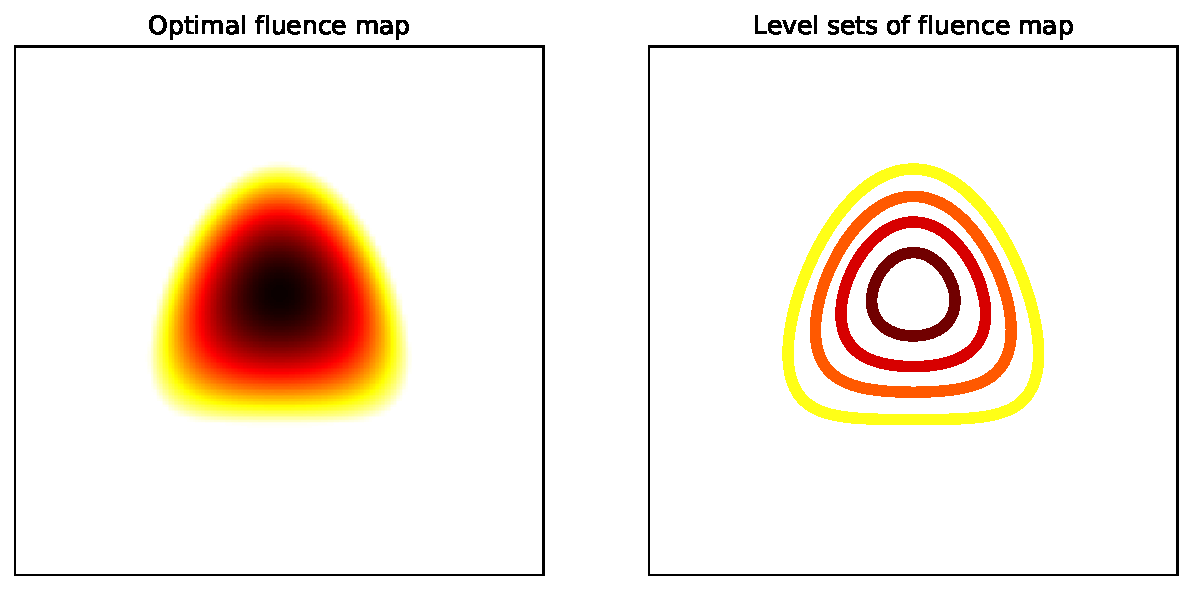
\includegraphics[height=4.5cm]{_fluence_map_discretization.pdf}
	\caption{Example of a fluence map discretization.}
	\label{fig:fluence_map_discretization}
\end{figure}
The fluence maps are divided into discrete levels (figure \ref{fig:fluence_map_discretization}).
\begin{figure}
	\centering
	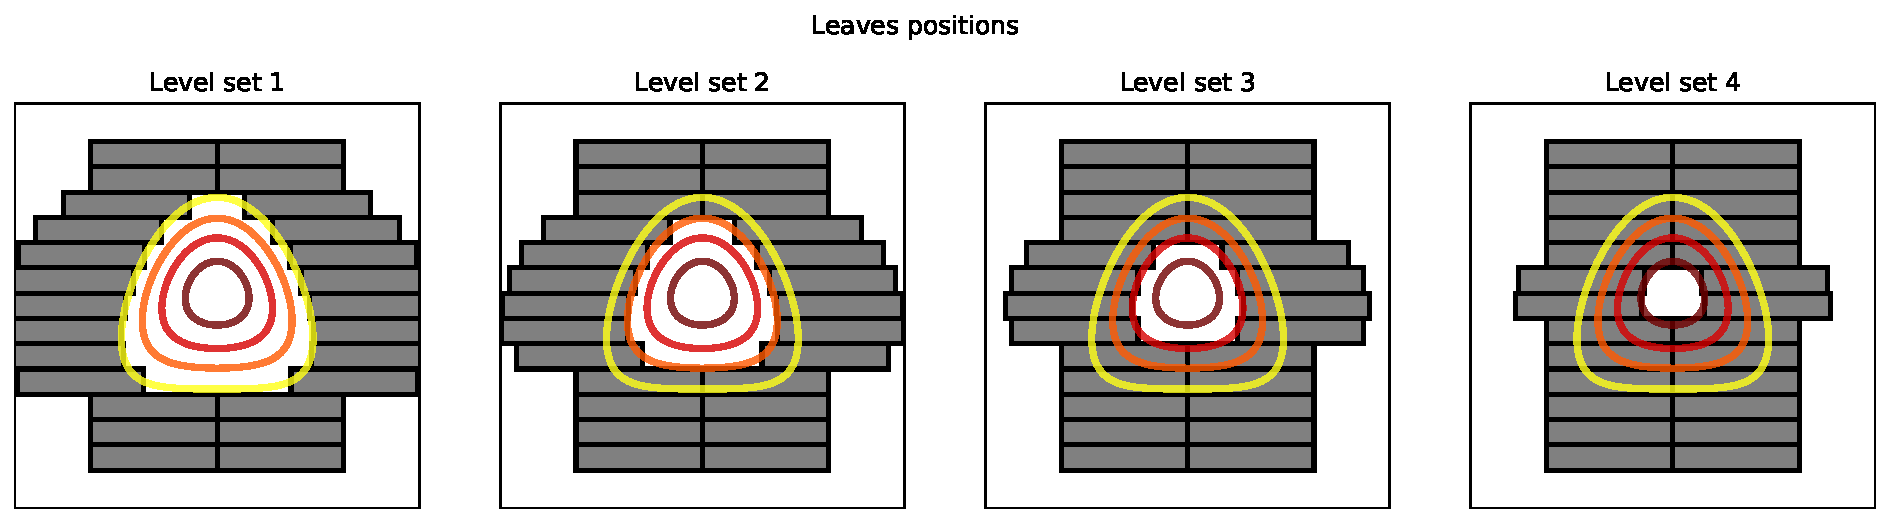
\includegraphics[height=4cm]{_level_set_matching_with_leaves.pdf}
	\caption{Example of level set matching with leaves.}
	\label{fig:level_set_matching_with_leaves}
\end{figure}
Then, the MLC leaves are positioned so that the open area of the irradiation head matches the level set (figure \ref{fig:level_set_matching_with_leaves}).
\begin{figure}
	\centering
	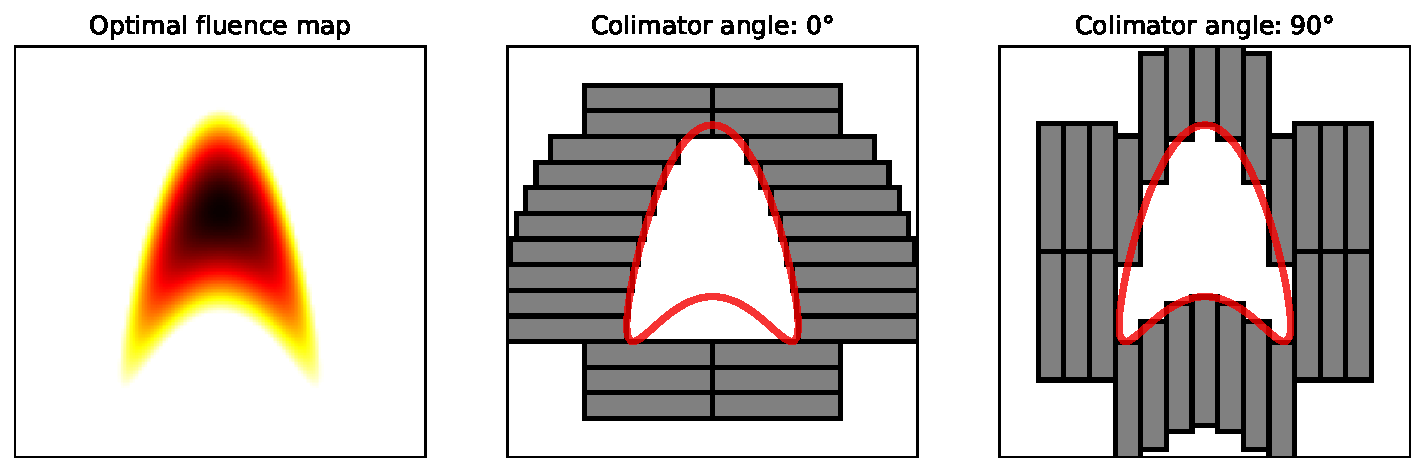
\includegraphics[height=4.2cm]{_leaves_angle.pdf}
	\caption{Example of a concave level matched with leaves.}
	\label{fig:leaves_angle}
\end{figure}
Note that convex level sets can all be matched with the MLC leaves; in case the level set is concave, changing the collimator angle may still allow the leaves to match the level set shape (figure \ref{fig:leaves_angle}).
Each level set is delivered as a static beam in sequence.
As the level sets are refined, the irradiation time increases
There is therefore a tradeoff to find between achieving greater accuracy and maintaining an efficient treatment time.

\paragraph[SW]{Sliding Window}
The "Sliding Window" technique, in contrast, is more computationally intensive:
The MLC leaves continuously move during beam delivery.
Finding the appropriate leaves motions requires solving a linear programming problem for each pair of leaves (sometimes called "Inverse Sliding Window Algorithm").
The fluence is segmented in one dimensional fluence curve along each leaf pair axis.
Correctly solving the linear programming problem allows a leaf pair to deliver any fluence within arbitrary approximation, in a reasonable amount of time.
A playground to calculate the leaves motion for an arbitrary fluence is available here:
\url{https://mics-lab.github.io/PresentationJuin2023PRFD/demo}.
% add playground demo for multi-leaf?

The sliding window technique is used most of the time, as delivery time is much (about twice) faster \cite{Ning2003}.

\subsection[DAO]{(Optional) Direct Aperture Optimization}
% mostly used for VMAT
% is sometimes used to fine tune IMRT



% %%%%%%%%%%%%%%%%%%%%%%%%%%%%%%%%%%%%%%%%%%%%%%%%%%%% %
% %%%%%%%%%%%%%%%%%%%%%%%%%%%%%%%%%%%%%%%%%%%%%%%%%%%% %
% %%%%%%%%%%%%%%%%%%%%%%%%%%%%%%%%%%%%%%%%%%%%%%%%%%%% %
% %%%%%%%%%%%%%%%%%%%%%%%%%%%%%%%%%%%%%%%%%%%%%%%%%%%% %
% %%%%%%%%%%%%%%%%%%%%%%%%%%%%%%%%%%%%%%%%%%%%%%%%%%%% %



\section{Simulation}
lots of approximations were made in the dosimetry, so there is a need to re-simulate to check that the machine instructions send a dose that is not too far from what was expected .
% https://oncologymedicalphysics.com/dose-calculation-algorithms/



% %%%%%%%%%%%%%%%%%%%%%%%%%%%%%%%%%%%%%%%%%%%%%%%%%%%% %
% %%%%%%%%%%%%%%%%%%%%%%%%%%%%%%%%%%%%%%%%%%%%%%%%%%%% %
% %%%%%%%%%%%%%%%%%%%%%%%%%%%%%%%%%%%%%%%%%%%%%%%%%%%% %
% %%%%%%%%%%%%%%%%%%%%%%%%%%%%%%%%%%%%%%%%%%%%%%%%%%%% %
% %%%%%%%%%%%%%%%%%%%%%%%%%%%%%%%%%%%%%%%%%%%%%%%%%%%% %



\section{Treatment Planning Systems}
Treatment Planning Systems (TPS) are the crucial tools that calculate the precise machine (MLC) motions according to the dosimetrists priorities and the irradiation technique chosen.

\subsection{Manufacturer}
%\columnratio{0.6}
%\begin{paracol}{2}
%	\paragraph{Eclipse\texttrademark\ (Varian)}
%	\ \\
%	Eclipse\texttrademark\ \cite{eclipse}, developed by Varian, is one of the most widely used TPS globally.
%	It supports VMAT with one or multiple arcs, and IMRT with any number of beams.
%	Eclipse\texttrademark\ integrates with Varian's suite of treatment machines, and integrates an automatic contouring tool \cite{eclipse_brochure}.
%	
%	\switchcolumn
%	
%	\begin{figure}[H]
%		\centering
%		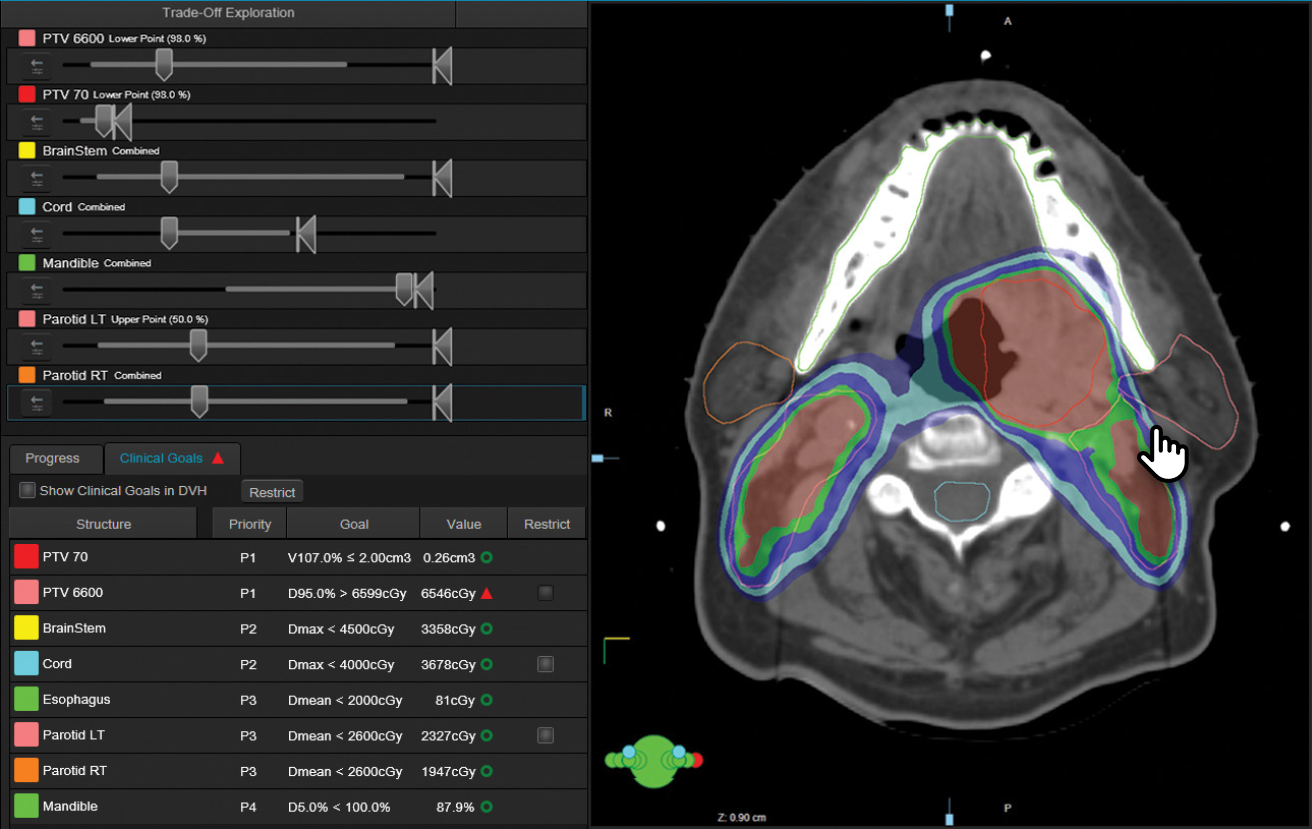
\includegraphics[width=\linewidth]{EclipseVarian.png}
%		\caption{Advertisement screenshot of \\ Eclipse\texttrademark\ (Varian's TPS).}
%		\label{fig:screenshot_eclipse}
%	\end{figure}
%\end{paracol}
\begin{multicols}{2}
	\paragraph{Eclipse\texttrademark\ (Varian)}
	\ \\
	Eclipse\texttrademark\ \cite{eclipse}, developed by Varian, is one of the most widely used TPS globally.
	It supports VMAT with one or multiple arcs, and IMRT with any number of beams.
	Eclipse\texttrademark\ integrates with Varian's suite of treatment machines, and integrates an automatic contouring tool \cite{eclipse_brochure}.
	
	\columnbreak
	
	\begin{figure}[H]
		\centering
		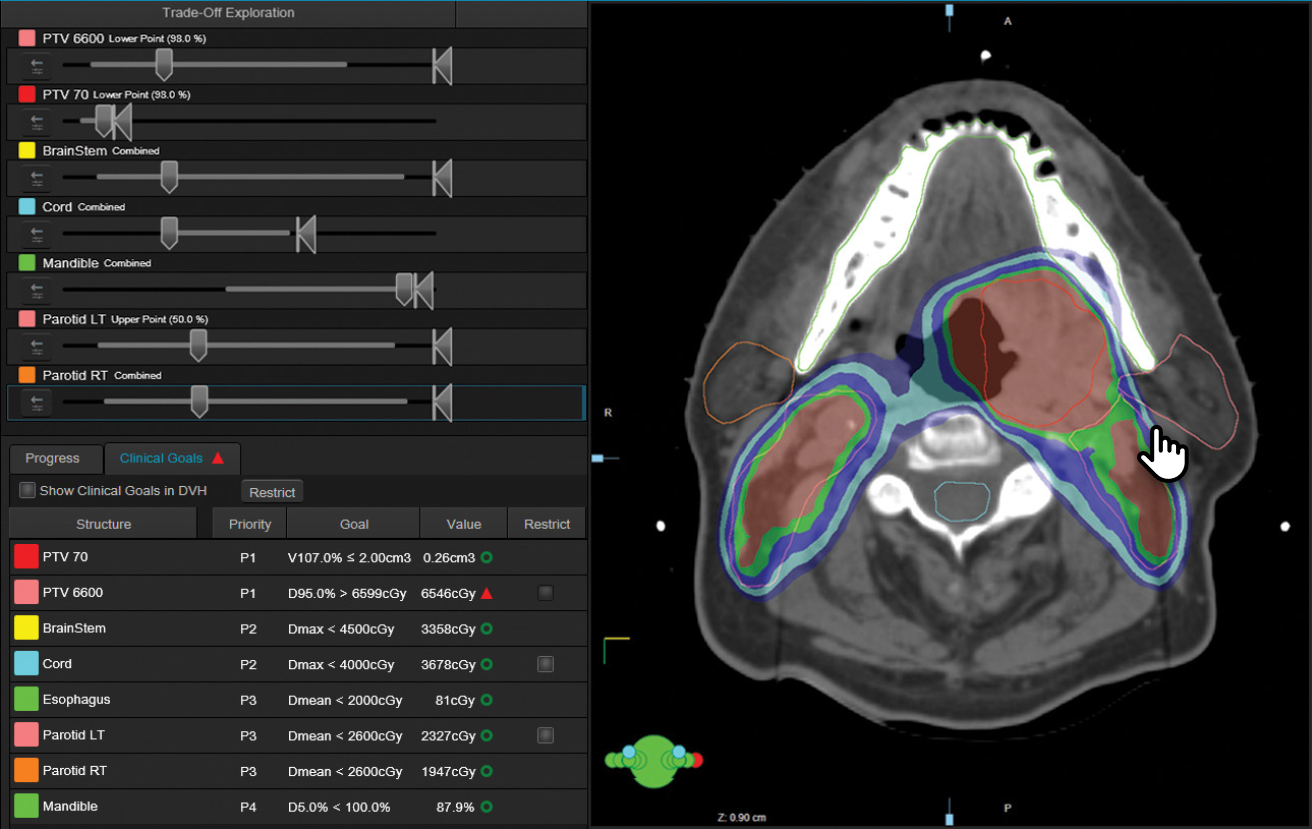
\includegraphics[width=\linewidth]{EclipseVarian.png}
		\caption{Advertisement screenshot of \\ Eclipse\texttrademark\ (Varian's TPS).}
		\label{fig:screenshot_eclipse}
	\end{figure}
\end{multicols}

\begin{multicols}{2}
	\paragraph{ONE® | Planning (Elekta)}
	\ \\
	ONE® | Planning \cite{one_planning} is Elekta's TPS, and is also widely used, supporting IMRT and VMAT.
	It is renowned for its speed with high-precision dose calculation using the Monte Carlo method.
	
	\columnbreak
	
	\begin{figure}[H]
		\centering
		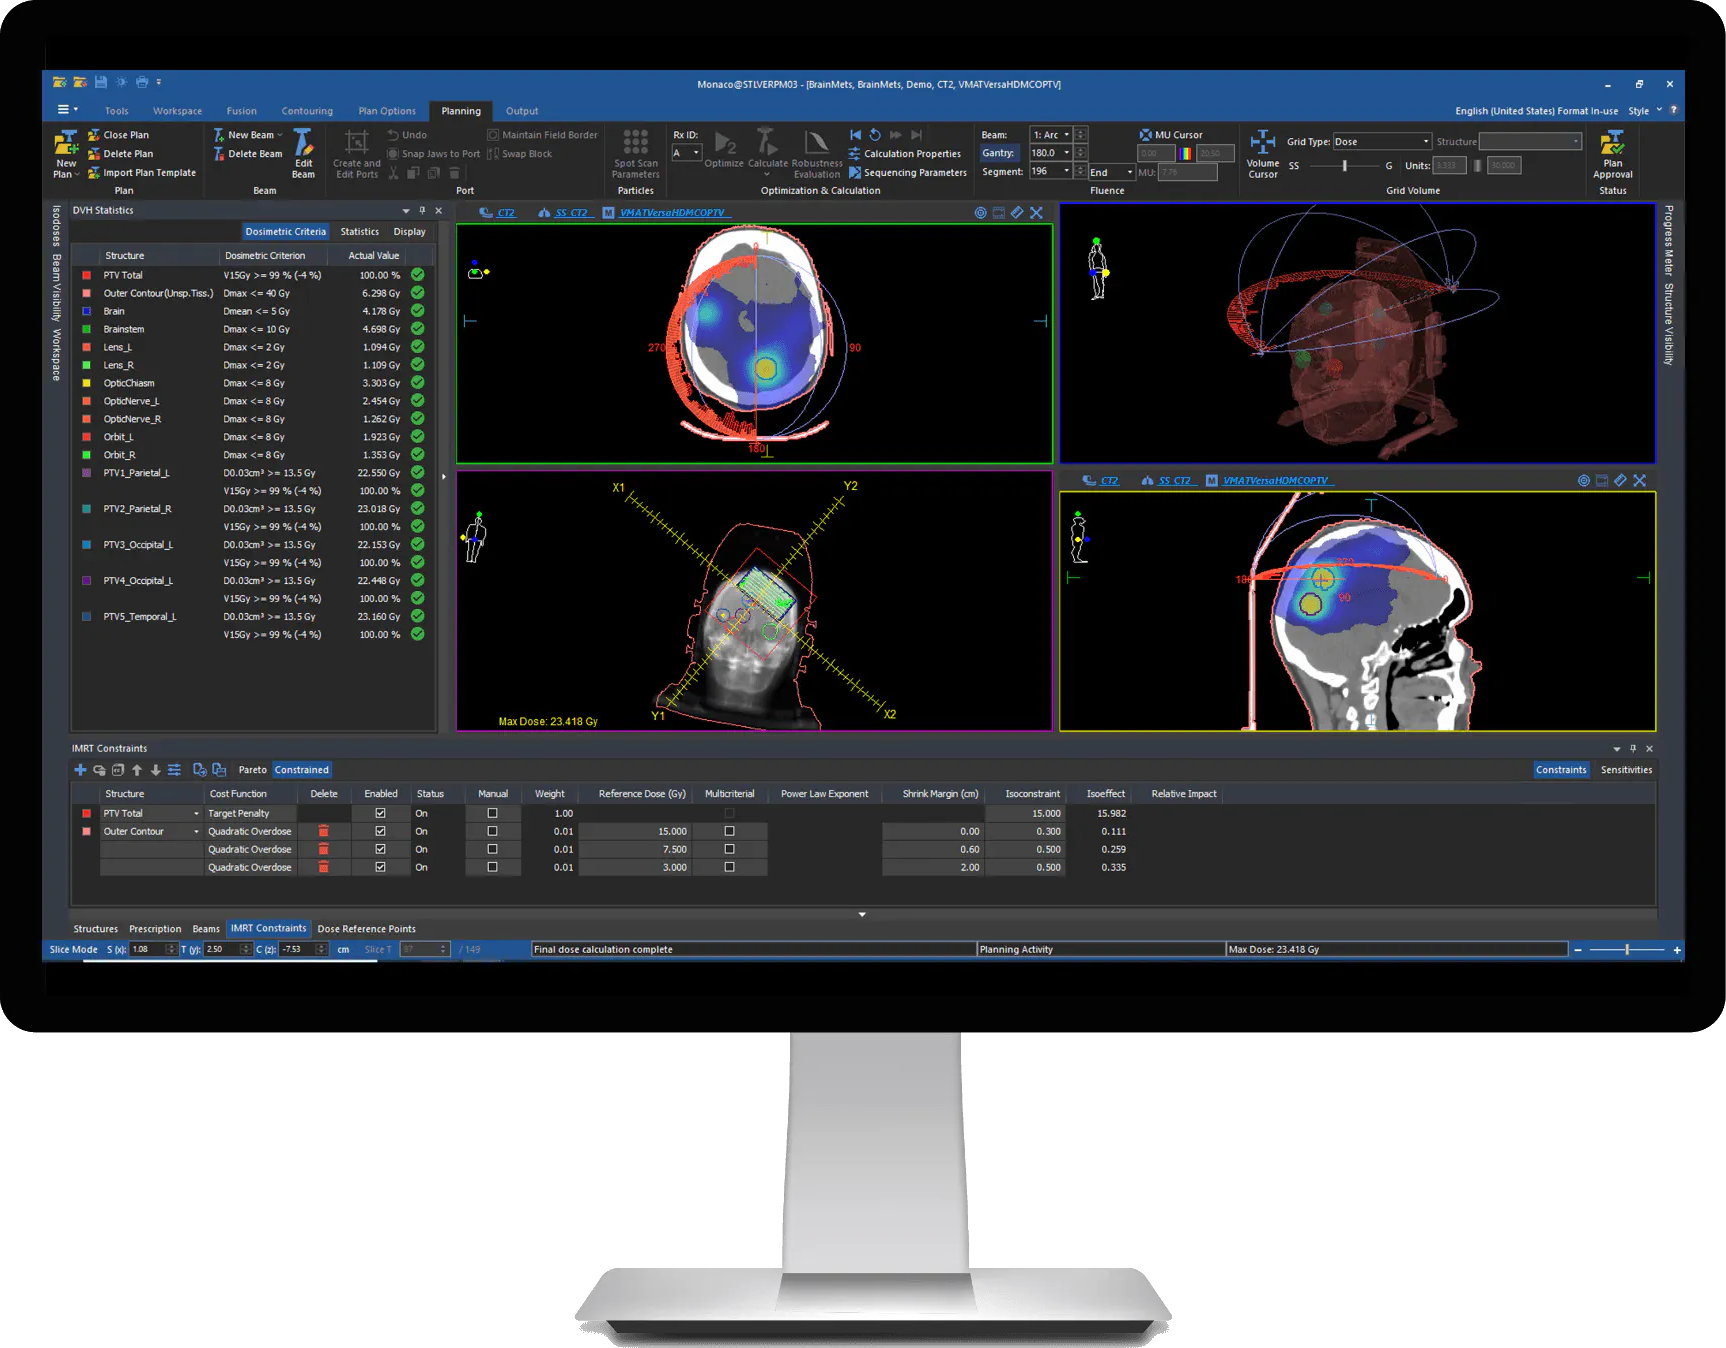
\includegraphics[width=\linewidth]{OnePlanningElekta.png}
		\caption{Advertisement screenshot of \\ ONE® | Planning (Elekta's TPS).}
		\label{fig:screenshot_one_planning}
	\end{figure}
\end{multicols}

\begin{multicols}{2}
	\paragraph{Precision® (Accuray)}
	\ \\
	Developed by Accuray, Precision® \cite{precision} is the dedicated TPS for CyberKnife and TomoTherapy systems.
	
	\columnbreak
	
	\begin{figure}[H]
		\centering
		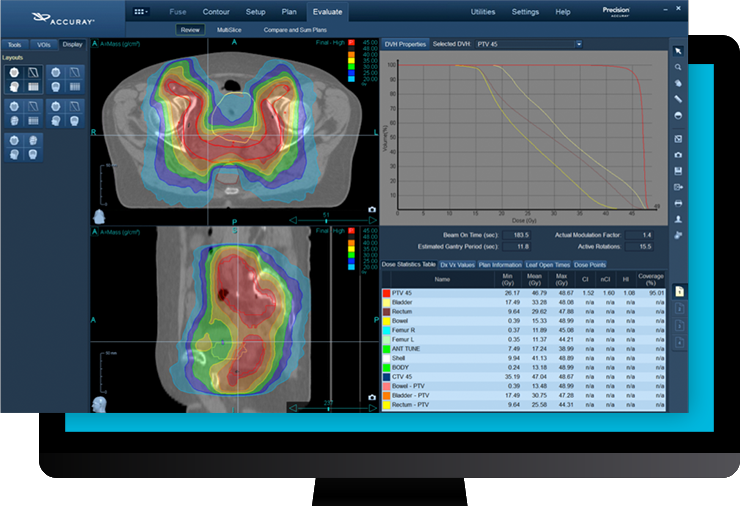
\includegraphics[width=\linewidth]{PrecisionAccuray.png}
		\caption{Advertisement screenshot of \\ Precision® (Accuray's TPS).}
		\label{fig:screenshot_precision}
	\end{figure}
\end{multicols}

\subsection{Non-manufacturer}
\begin{multicols}{2}
	\paragraph{RayStation (RaySearch)}
	\ \\
	RayStation \cite{raystation}, developed by RaySearch Laboratories, is a TPS known for its advanced optimization algorithms.
	Unlike manufacturer-specific systems, RayStation can output plans for a wide range of linear accelerators and imaging devices.
	It offers robust support for various treatment techniques, including VMAT, IMRT, 3D-CRT, Cyberknife, and TomoTherapy.
	
	\columnbreak
	
	\begin{figure}[H]
		\centering
		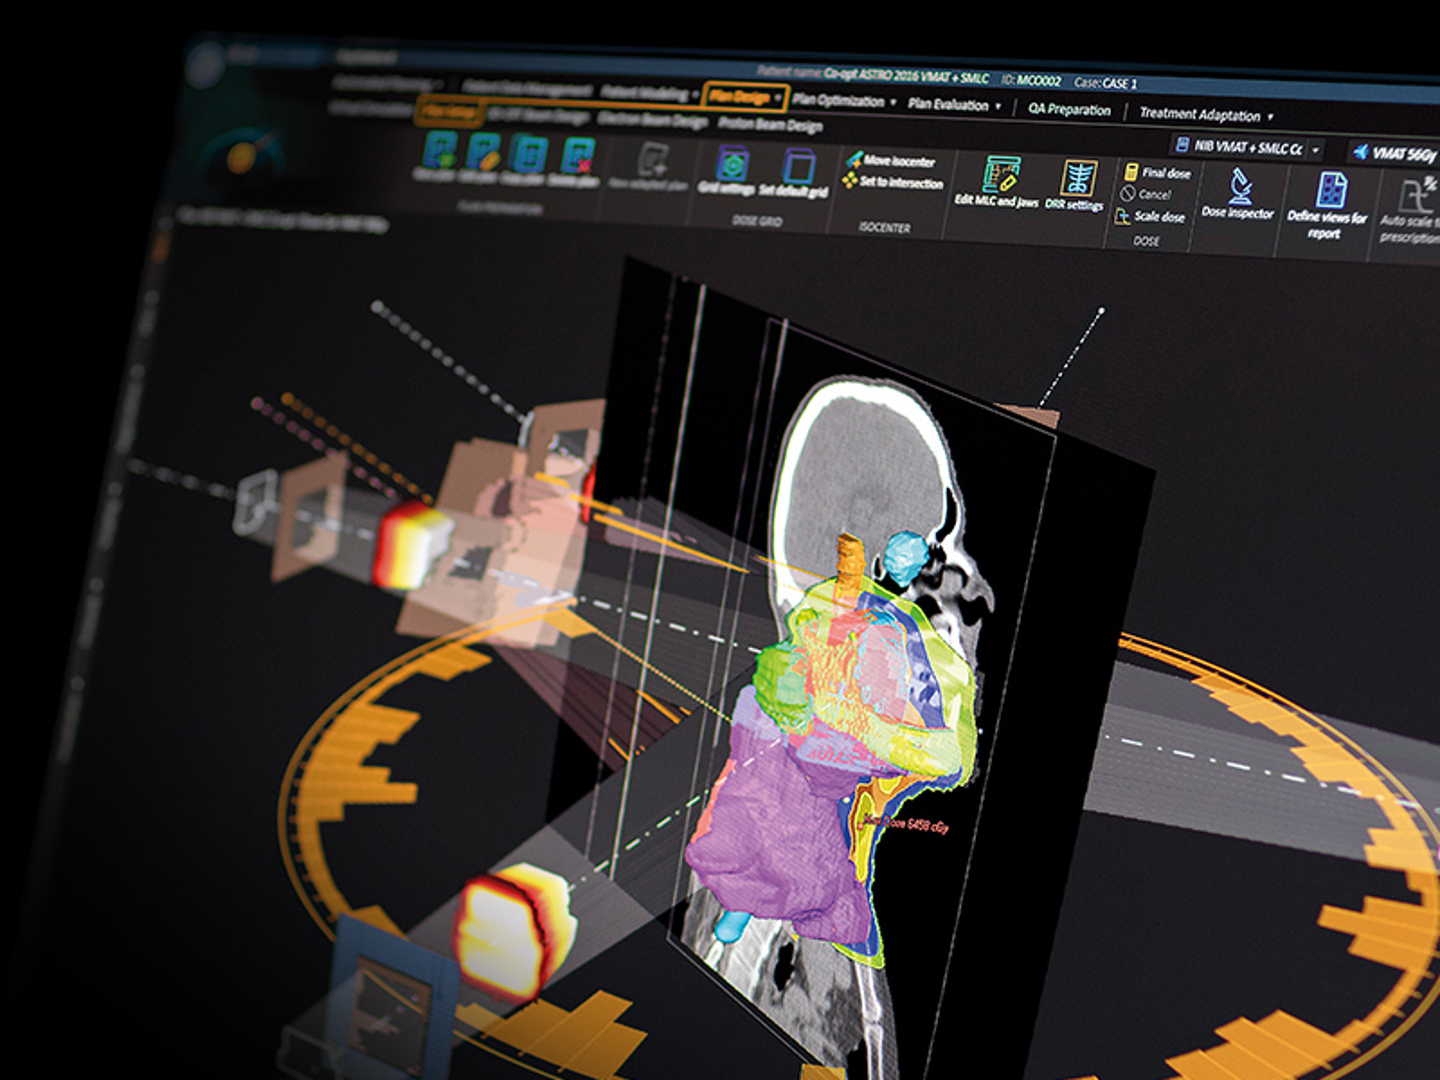
\includegraphics[width=\linewidth]{RaySearchRayStation.png}
		\caption{Advertisement screenshot of \\ RayStation (RaySearch's TPS).}
		\label{fig:screenshot_raysearch}
	\end{figure}
\end{multicols}

\begin{wrapfigure}{r}{0.3\textwidth}
	\vspace{-0.5cm}
	\centering
	
\includegraphics[width=0.3\textwidth]{matRad.png}
	\caption{matRad Logo}
	\label{fig:matRad_logo}
	\vspace{-0.5cm}
\end{wrapfigure}
\paragraph{matRad (German Cancer Research Center - DKFZ)}
\ \\
matRad \cite{matrad} is an open-source TPS developed by the German Cancer Research Center (DKFZ) for research and education.
While not intended for clinical use, matRad offers a flexible platform for testing and developing new treatment-planning algorithms.

\paragraph{AutoPlan (TheraPanacea - Unpublished)}
\ \\
AutoPlan is the upcoming TPS from TheraPanacea, designed to incorporate artificial intelligence and machine learning into the treatment planning process.


	
	\chapter{Introduction}
	\begin{chapterabstract}
		\lipsum[1-2]
	\end{chapterabstract}
	\clearpage
	\localtableofcontents
	\section{Context}
Cancer remains one of the leading causes of mortality worldwide, with its incidence projected to rise in the coming decades \cite{Quante2016,Smittenaar2016}.
As our understanding of cancer biology evolves and diagnostic techniques improve, the demand for effective and personalized treatment strategies continues to grow \cite{Howard2017}.
Radiotherapy has emerged as a cornerstone in cancer management, either as a standalone treatment or in combination with other modalities such as surgery, chemotherapy, and immunotherapy \cite{Rivoirard2015,Reynders2015}.
Radiotherapy leverages ionizing radiation to damage cancer cells' DNA, impeding their ability to proliferate and ultimately leading to cell death \cite{Yard2015}.
The efficacy of radiotherapy lies in its ability to deliver precise doses of radiation to tumor volumes while minimizing exposure to surrounding healthy tissues \cite{Malicki2012}.
This delicate balance between tumor control and normal tissue toxicity underscores the importance of treatment planning in radiotherapy \cite{Das2009}.

The advent of advanced imaging technologies \cite{Li_Zhang_2024}, coupled with sophisticated delivery systems like Multi-Leaf Collimator Linear Accelerators (MLC-LINACs), Tomotherapy units, and CyberKnife systems, has revolutionized the field of radiation oncology \cite{Klein_2009,Xia2001}.
These technological advancements have paved the way for highly conformal treatment techniques.
Intensity-Modulated Radiation Therapy (IMRT) and Volumetric Modulated Arc Therapy (VMAT) techniques offer unprecedented levels of dose sculpting, allowing for escalated doses to tumors while better sparing organs at risk \cite{Ng2018,Elith2011,Davidson2011}.
However, the increased complexity of modern radiotherapy techniques has led to a corresponding increase in the complexity of treatment planning \cite{Fraass2012,Robinson2008}.
The process of creating an optimal treatment plan involves multiple steps, including Beam Orientation Optimization (BOO) \cite{Pugachev2000,Pugachev2001}, Fluence Map Optimization (FMO) \cite{Lim2008,Romeijn_2004,Lee2006}, Leaf Sequencing (LS) \cite{Chen2003,Chen2005,Xia2002}, and (sometimes) Direct Aperture Optimization (DAO) \cite{Shepard2002,Earl_2003,Ahunbay2007}.
Each step requires careful consideration of numerous variables and constraints, making the planning process time-consuming and labor-intensive \cite{Wang2019}.

In this context, this thesis aims to explore and advance the radiotherapy treatment planning automation field, focusing on developing novel algorithms and methodologies to enhance treatment plans' efficiency, quality, and consistency.
By building upon the foundational knowledge of radiotherapy physics, biology, and clinical workflow, we seek to contribute to the ongoing evolution of radiation oncology and, ultimately, to improve outcomes for cancer patients.

\section{Problematic}
Traditional manual radiotherapy planning procedures are inherently subjective and time-consuming.
The reliance on individual planner expertise often leads to variability in treatment plan quality\cite{Chung2008,Bohsung2005,Das2008,Williams2007}.
This treatment plan diversity can induce inconsistencies in patient care.
While efforts have been made to enhance consistency \cite{Bahm2011}, significant variability among planners and institutions persists.
There is a pressing need for more standardized planning approaches.
The automation of treatment planning processes presents a promising solution to these challenges.

Moreover, the time-intensive nature of manual optimization \cite{Zhang2020} and the growing demand for radiotherapy services have created a pressing need to develop automated approaches to streamline the radiotherapy planning process.
Automation enables the treatment of more patients and facilitates exploring a broader range of treatment options.

By applying computational algorithms and artificial intelligence, automated planning systems offer the potential to enhance radiotherapy treatment delivery significantly.
These systems can improve patient throughput and resource allocation by reducing planning time and increasing departmental efficiency.
Automated planning can improve plan quality and consistency, reducing variability and ensuring optimal treatment outcomes.
Furthermore, the ability to enable rapid re-planning facilitates adaptive radiotherapy, allowing for adjustments to treatment plans in response to changes in tumor volume or patient anatomy.
Finally, automated systems can explore a more expansive solution space, potentially discovering novel and innovative planning strategies that may improve treatment outcomes.

However, the development and implementation of automated planning systems pose challenges.
These challenges include the creation of robust optimization algorithms, integrating with existing Treatment Planning Systems, and validating against current clinical standards.

\section{State of the Art}
\paragraph{Knowledge-based radiotherapy planning}
Knowledge-based radiotherapy planning (KBRP) represents an objective methodology for incorporating patient-specific data and historical experience into the treatment planning process \cite{Nwankwo_2014}.
By automating the optimization of KBRP, it is anticipated that a viable alternative to the current human-centric treatment planning paradigm can be established.
A prevalent KBRP approach involves leveraging a database of historical benchmark plans to learn patient-specific dosimetric parameters and generate new treatment plans.
Automated KBRP tools effectively set optimization parameters based on the desired dose-volume histogram.
Previous studies have reported notable dosimetric improvements in treatment plans generated by KBRP approaches compared to benchmark data, particularly regarding sparing organs at risk \cite{Fogliata2014,Tol2015}.

\paragraph{Conventional techniques}

\paragraph{Pareto surface exploration}
In DVH-based inverse optimization used by most commercial TPS, a cost function must be defined to solve the minimization problem.
This function combines data from all volumes of interest as a weighted sum of penalties from each DVH constraint.
The weighting coefficients reflect trade-offs between the target(s) and different OARs.
However, this approach requires reoptimization if dosimetric preferences change during plan evaluation, making it time-consuming to find the optimal balance.
To address this, multi-criteria optimization (MCO) was introduced, enabling the simultaneous generation of multiple "anchor" plans.
Each anchor plan optimizes one OAR’s DVH criterion for maximal sparing without compromising tumor target dosimetry.
These plans form a hypersurface in the $N$-dimension space, where $N$ is the number of independent OAR dosimetric constraints.
Referred to as the Pareto surface, this hypersurface contains the optimal plans following different dosimetric criteria.

Previous research has explored Pareto optimal tradeoffs in various domains.
Gebru et al., for instance, investigated methods for evaluating Pareto optimality \cite{Gebru2023}.
Similarly, Cilla et al. conducted a comprehensive analysis of Pareto fronts \cite{Cilla2018}.
These studies provide valuable insights into the principles and techniques associated with Pareto optimization.
Craft et al. proposed a method for generating multiple Pareto optimal dose distributions, allowing clinicians to make informed decisions based on their specific preferences and clinical contexts \cite{Craft2007}

\section{Unsolved problems}
Numerous approaches have been investigated to automate the radiotherapy treatment planning process.
Despite these efforts, a consensus on the optimal method has yet to be established, and few automated solutions have been adopted in clinics.
The challenges associated with automating radiotherapy treatment planning remain a significant area of inquiry within the field.
This thesis addresses this critical issue by proposing advancements in key areas that may contribute to developing a fully automated treatment planning system.

\section{Thesis overview}
This section provides a comprehensive summary of the forthcoming chapters of this thesis.

\subsection{Fluence Map Optimization}
Chapter 3 is dedicated to developing computational methods for Fluence Map Optimization (FMO).
The chapter begins by assessing the discretization strategies.
Naive approaches for optimization are explored, stepping up to a formalization of the classical FMO problem.
A significant focus is placed on incorporating medical constraints and the corresponding importance factors associated with each constraint, which are critical in ensuring clinically viable treatment plans.
The performance of various optimization algorithms is evaluated and compared, providing insights into their relative efficiencies in solving the FMO problem.
This primary work was published in the form of an ArXiV article.

\subsection{Semi-automation}
\subsubsection*{Using graph-based analysis}
Chapter 4 explores the interrelationships between radiotherapy treatment plans by defining a distance metric.
This distance is then used to cluster plans into meaningful groups.
The clustering forms a basis for developing a semi-automated framework for treatment plan optimization.
Leveraging graph-based methodologies, this approach reduces the need for manual intervention in the planning process while ensuring the generation of high-quality plans.
The potential of this semi-automated framework to streamline clinical workflows was presented at the 2024 European Society for Radiotherapy and Oncology (ESTRO) conference.

\subsection{Full-automation}
\subsubsection*{With reinforcement learning and conventional treatment optimization techniques}
Chapter 5 addresses the limitations of classical optimization techniques in fully automating the treatment planning process.
This chapter introduces a novel framework that integrates reinforcement learning with conventional optimization.
The reinforcement learning agent is driven by clinical expertise and can be specialized to center-specific guidelines.
The findings from this work have been disseminated through a peer-reviewed journal article, a presentation at the Artificial Intelligence in Medicine (AIME) 2024 conference, and a poster presentation at the American Society for Radiation Oncology (ASTRO) 2024 meeting.

\subsection{Hybrid-automation}
\subsubsection*{Via target DVHs deep dose and dose mimicking technique}
The final research chapter, Chapter 6, presents a hybrid approach to automating treatment planning.
This approach combines deep learning for dose prediction with target Dose-Volume Histograms (DVHs) and plan-mimicking strategies.
This methodology bridges the gap between fully automated AI-driven techniques and traditional planning methods, offering a more adaptable and clinically feasible solution.
The hybrid model provides a mechanism for mimicking high-quality plans from experienced planners.
This research has been presented at the French Society of Medical Physics (SFPM) and the French Society for Radiation Oncology (SFRO) 2024 meetings.

	
	\chapter{Dosimetry Optimization}
	\begin{chapterabstract}
	\end{chapterabstract}
	\clearpage
	\localtableofcontents
	\section{Optim engine: classic and dose mimicking}
	\section{relation between optim doses (distance and network)}
	\section{ESTRO (novel approach with graph theory)}
	
	\chapter{Automation: Classical Approach}
	\begin{chapterabstract}
	\end{chapterabstract}
	\clearpage
	\localtableofcontents
	\section{RL + classic optim algo (AIME / ASTRO)}
	
	\chapter{Automation: Deep Dose}
	\begin{chapterabstract}
	\end{chapterabstract}
	\clearpage
	\localtableofcontents
	\section{DVH guided deep dose + dose mimicking algo (SFPM / SFRO)}
	
	\chapter{Conclusion}
	\chapter{Perspectives}
	

\end{document}
